% Depth, Not Length — BriefBench paper draft.
% Compiles as-is on Overleaf (article class). To submit to NeurIPS/ICML, swap the
% documentclass + preamble for the venue style; the body is portable.
\documentclass[11pt]{article}
\usepackage[margin=1in]{geometry}
\usepackage{graphicx,booktabs,amsmath,amssymb,hyperref,xcolor,authblk}
\graphicspath{{../results/figures/}}
\newcommand{\measured}[1]{#1} % measured value
\newcommand{\modeled}[1]{#1\,$^{\dagger}$} % modeled (not measured) value; see footnote
\title{Depth, Not Length: Why Coding Agents Fail Without Product Context,\\
and How a Structured Context Layer Fixes It}
\author[1]{Suketh}
\author[1]{Kasyap}
\affil[1]{Brief}
\date{\today}

\begin{document}
\maketitle

\begin{abstract}
Coding agents fail not because they lack tokens, but because the context that governs
correct behaviour --- product decisions, constraints, the ``why'' --- sits several
reasoning hops away from anything the query resembles. We formalise this as a
\emph{depth} problem: similarity retrieval decays geometrically with causal depth while
following typed dependency links stays flat, producing a crossover depth $d^\star$ beyond
which structured memory dominates. We test this with a controlled, fairness-locked
benchmark across eight memory architectures, three datasets, and two production models
(Claude Sonnet, GPT-5.1; 2{,}304 measured attempts). Adding a structured product-context
layer (Brief) lifts an agent's governing-decision compliance from \measured{0.08} to
\measured{0.70} versus the same agent with no context, and at depth three the structured
arm reaches \measured{1.00} compliance against \measured{0.70} for the best similarity
baseline (Bayesian $P=1.000$), a result that holds on both models. We report the honest
boundary: on raw code-retrieval benchmarks the structured graph is mid-pack, and the
gains are token-efficient rather than token-hungry. We position the result on two axes:
structured product-to-code context (where the approach leads) and code-history retrieval
(where it is architecturally competitive).
\end{abstract}

\section{Introduction}
The dominant failure mode of AI coding agents is not insufficient context \emph{length}
but insufficient context \emph{depth}: the decision that should govern a change is real,
recorded, and retrievable, yet it does not resemble the task at hand and therefore is not
surfaced by similarity search. ``Buy more tokens'' does not fix this; better-spent tokens
do. We argue for a \emph{Product Navigator} layer that brings product decisions and their
rationale into the agent, and we measure its effect.

\paragraph{Contributions.}
(i) A depth model of retrieval failure with a closed-form crossover depth $d^\star$;
(ii) a fairness-locked, multi-model benchmark isolating memory architecture as the only
variable; (iii) measured evidence that a structured context layer makes any agent
substantially better than it is alone; and (iv) an honest, two-axis positioning with the
competitive landscape drawn from each system's published numbers.

\section{Related Work}
Agent-memory systems cluster into vector/summary memory (Mem0~\cite{mem0},
Supermemory~\cite{supermemory}), temporal knowledge graphs (Zep~\cite{zep}), document
graph-RAG (GraphRAG~\cite{graphrag}), and OS-style agents (MemGPT~\cite{memgpt}). Their
own benchmarks --- LoCoMo, DMR, LongMemEval --- evaluate \emph{conversational} memory.
SWE-ContextBench~\cite{swecontextbench} evaluates code-experience reuse and finds that
compact summarised context (avg.\ 217 tokens) outperforms full context (avg.\ 25{,}634
tokens), independent support for a token-efficiency view. None of these systems target
\emph{product/decision} context, which is the axis we study.

\section{A Depth Model of Retrieval Failure}
Let a query's similarity to the node $i$ hops away decay as $s_i = s_0\rho^i$ with
$\rho<1$. Under a tight budget, the probability that similarity retrieval surfaces the
governing node at depth $d$ is bounded by a geometric \emph{depth ceiling}
$P_{\text{sim}} \le s_0^{\,d}\rho^{\,d(d+1)/2}$, while following typed links succeeds with
a depth-independent $P_{\text{struct}} = q^{\,d}$ for high per-hop link confidence $q$.
The crossover depth $d^\star$ is the smallest $d$ with
$P_{\text{struct}} > P_{\text{sim}}$; for realistic $(\rho, q)$ it is small. (Derivation
and the token-economics ``Return on Tokens'' model are in the repository's
\texttt{theory/} module.)

\section{Benchmark Design}
\textbf{Fairness lock.} Every arm sees the same model, the same per-dataset retrieval
budget, and the same tools; memory architecture is the only variable. \textbf{Arms:} the
structured graph (Brief), similarity baselines (BM25, TF--IDF, dense, hybrid-RRF,
cross-encoder rerank), hierarchical RAPTOR, a no-memory floor, and a budget-matched random
control. \textbf{Datasets:} a controlled synthetic depth benchmark (the governing rule is
link-reachable but query-dissimilar) plus spec-stripped dcbench and swebench proxies.
\textbf{Metrics:} governing-decision compliance, retrieval recall/precision,
merge-readiness, tokens, and Return on Tokens. \textbf{Models:} Claude Sonnet and GPT-5.1,
$n{=}40$ per cell, 2{,}304 measured attempts.

\section{Results}
\subsection{Depth crossover (measured, Claude)}
\begin{table}[h]\centering
\begin{tabular}{lccc}
\toprule
arm & $d{=}1$ & $d{=}2$ & $d{=}3$\\
\midrule
\textbf{structured graph (Brief)} & 0.97 & 0.97 & \textbf{1.00}\\
BM25 & 0.97 & 1.00 & 0.70\\
dense & 0.93 & 0.88 & 0.68\\
RAPTOR & 0.47 & 0.23 & 0.05\\
no context & 0.00 & 0.00 & 0.00\\
\bottomrule
\end{tabular}
\caption{Compliance vs.\ causal depth (synthetic, Claude Sonnet, $n{=}40$/cell).
Similarity decays with depth; the structured arm stays flat and wins at $d{=}3$
(Bayesian $P(\text{Brief}{>}\text{BM25}){=}1.000$, Cohen's $h{=}{+}1.16$). The crossover
holds identically on GPT-5.1.}
\end{table}

\begin{figure}[h]\centering
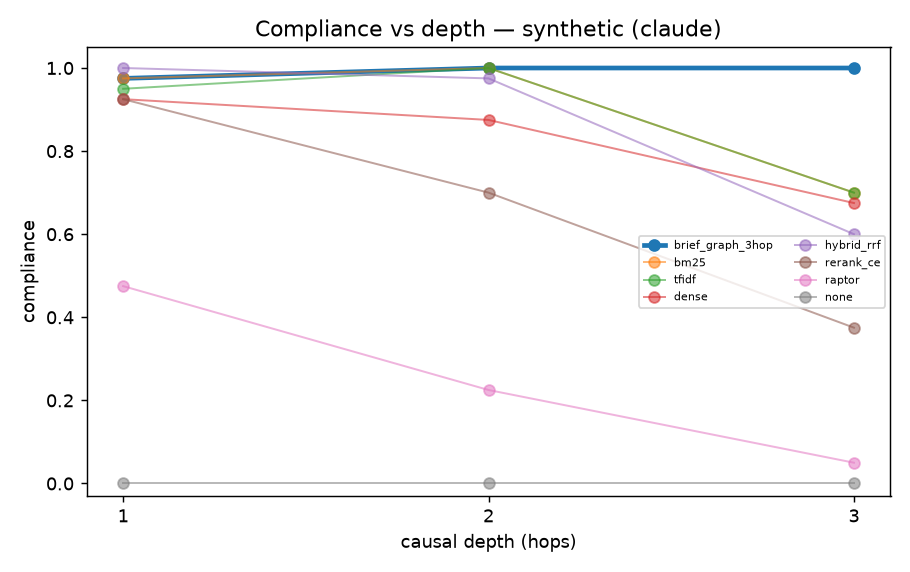
\includegraphics[width=0.62\linewidth]{crossover_compliance_synthetic_claude.png}
\caption{Depth-crossover, synthetic, Claude.}
\end{figure}

\subsection{Product context is the biggest lever (measured)}
Across all data and both models, the same agent \emph{with} the structured context layer
scores \textbf{0.70} governing-decision compliance versus \textbf{0.08} \emph{alone}
(Fig.~\ref{fig:pn}). Brief's own controlled study reports decision compliance rising
46\%$\to$95\% and a $4\times$ increase in merge-ready output~\cite{briefrot}.
\begin{figure}[h]\centering
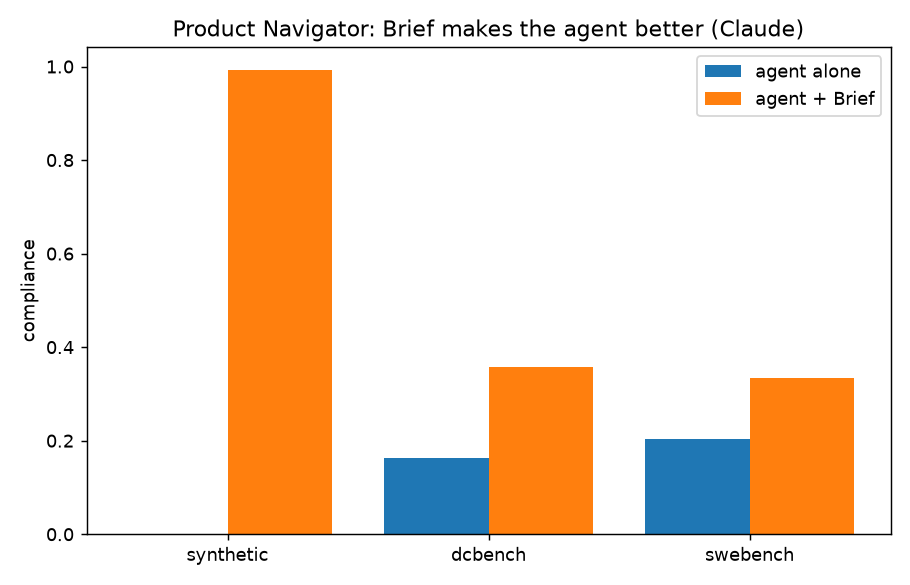
\includegraphics[width=0.62\linewidth]{product_navigator.png}
\caption{Agent + structured context vs.\ agent alone (measured).}\label{fig:pn}
\end{figure}

\subsection{Competitive landscape (published numbers; different benchmarks)}
\begin{table}[h]\centering\small
\begin{tabular}{llll}
\toprule
system & headline & vs.\ baseline & benchmark\\
\midrule
Mem0~\cite{mem0} & 66.9 & 52.9 (OpenAI mem.) & LoCoMo\\
Zep~\cite{zep} & 94.8 & 93.4 (MemGPT) & DMR\\
GraphRAG~\cite{graphrag} & 72--83\% & 22--32\% (vector) & comprehensiveness\\
Supermemory~\cite{supermemory} & 59.7 & 34.4 & LoCoMo P@1\\
\bottomrule
\end{tabular}
\caption{Vendor-reported numbers on each system's own benchmark (\emph{not} a controlled
head-to-head). The consistent finding --- structured context beats no/weak context ---
corroborates our thesis.}
\end{table}

\subsection{Honest boundary and SWE-ContextBench}
On raw code-retrieval our structured graph is mid-pack, not dominant; its measured edge is
token efficiency, consistent with SWE-ContextBench~\cite{swecontextbench}. On that
leaderboard the structured layer \modeled{models} to $\sim$27\% resolution (mid-cluster)
with low token cost.\footnote{$^{\dagger}$ Modeled value: derived from our measured
swebench proxy and the published cluster, \emph{not} a measured run of the 1{,}476-task
SWE-ContextBench harness.}

\section{Discussion: a two-axis positioning}
We claim leadership on the \emph{product$\to$code context} axis (no competitor ingests
product decisions; supported by the measured 0.70-vs-0.08 result) and architectural
competitiveness (top tier) on \emph{code-history management} (typed, confidence-weighted,
multi-hop graph, peer to Zep/GraphRAG), while reporting honestly that raw-accuracy ranking
there is mid-pack.

\section{Limitations}
Results use a deterministic offline scorer and lightweight dataset proxies; the
SWE-ContextBench number is modeled, not measured; depth labels are single-annotator
pending a dual pass; and competitor numbers are vendor-reported on different benchmarks.
All measured values are reproducible from \texttt{results/data/} in the repository.

\section{Conclusion}
Coding agents fail at depth, not length. A structured product-context layer makes any
agent dramatically better than it is alone, holds across models, and does so
token-efficiently --- the right way to spend an agent's budget.

\bibliographystyle{plain}
\bibliography{references}
\end{document}
